% Section 3

2. \textbf{Robot Butler:} 
A simulation of a robot butler in an office building, where the robot's task is 
to navigate between two rooms to serve drinks to two people. These people can 
have the role of a salesperson, engineer, or manager, and the rooms can each be 
an office space, conference room, kitchen, or workshop. Additionally, it can be 
early or late in the week and the people can be using equipment at a location. 
This domain has only \~40 permutations of its physical object properties and 4 
actions in a standard MDP formulation, but has ~1150 static configurations. 
Figure~\ref{fig:robotbutler} is a partial illustration of one state of the MDP. 

\begin{figure}[t]
  \centerline{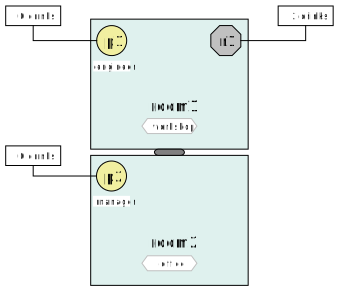
\includegraphics[width=2.5in]{robot-butler-domain}}
  \caption{Example of a scenario in the Robot Butler domain. Depicted is the 
  physical configuration of objects in the domain, as well as static attributes 
  \textit{room type} and \textit{person role}.}
\label{fig:robotbutler} 
\vspace{1mm}
\end{figure}

%%%%%%%%%%%%%%%%%%%%%%%%%%%%%%%%

% Section 3.1



%%%%%%%%%%%%%%%%%%%%%%%%%%%%%%%%



